% Options for packages loaded elsewhere
% Options for packages loaded elsewhere
\PassOptionsToPackage{unicode}{hyperref}
\PassOptionsToPackage{hyphens}{url}
\PassOptionsToPackage{dvipsnames,svgnames,x11names}{xcolor}
%
\documentclass[
  11pt,
  letterpaper,
]{article}
\usepackage{xcolor}
\usepackage[margin=1in,headheight=14pt]{geometry}
\usepackage{amsmath,amssymb}
\setcounter{secnumdepth}{-\maxdimen} % remove section numbering
\usepackage{iftex}
\ifPDFTeX
  \usepackage[T1]{fontenc}
  \usepackage[utf8]{inputenc}
  \usepackage{textcomp} % provide euro and other symbols
\else % if luatex or xetex
  \usepackage{unicode-math} % this also loads fontspec
  \defaultfontfeatures{Scale=MatchLowercase}
  \defaultfontfeatures[\rmfamily]{Ligatures=TeX,Scale=1}
\fi
\usepackage{lmodern}
\ifPDFTeX\else
  % xetex/luatex font selection
\fi
% Use upquote if available, for straight quotes in verbatim environments
\IfFileExists{upquote.sty}{\usepackage{upquote}}{}
\IfFileExists{microtype.sty}{% use microtype if available
  \usepackage[]{microtype}
  \UseMicrotypeSet[protrusion]{basicmath} % disable protrusion for tt fonts
}{}
\makeatletter
\@ifundefined{KOMAClassName}{% if non-KOMA class
  \IfFileExists{parskip.sty}{%
    \usepackage{parskip}
  }{% else
    \setlength{\parindent}{0pt}
    \setlength{\parskip}{6pt plus 2pt minus 1pt}}
}{% if KOMA class
  \KOMAoptions{parskip=half}}
\makeatother
% Make \paragraph and \subparagraph free-standing
\makeatletter
\ifx\paragraph\undefined\else
  \let\oldparagraph\paragraph
  \renewcommand{\paragraph}{
    \@ifstar
      \xxxParagraphStar
      \xxxParagraphNoStar
  }
  \newcommand{\xxxParagraphStar}[1]{\oldparagraph*{#1}\mbox{}}
  \newcommand{\xxxParagraphNoStar}[1]{\oldparagraph{#1}\mbox{}}
\fi
\ifx\subparagraph\undefined\else
  \let\oldsubparagraph\subparagraph
  \renewcommand{\subparagraph}{
    \@ifstar
      \xxxSubParagraphStar
      \xxxSubParagraphNoStar
  }
  \newcommand{\xxxSubParagraphStar}[1]{\oldsubparagraph*{#1}\mbox{}}
  \newcommand{\xxxSubParagraphNoStar}[1]{\oldsubparagraph{#1}\mbox{}}
\fi
\makeatother


\usepackage{longtable,booktabs,array}
\usepackage{calc} % for calculating minipage widths
% Correct order of tables after \paragraph or \subparagraph
\usepackage{etoolbox}
\makeatletter
\patchcmd\longtable{\par}{\if@noskipsec\mbox{}\fi\par}{}{}
\makeatother
% Allow footnotes in longtable head/foot
\IfFileExists{footnotehyper.sty}{\usepackage{footnotehyper}}{\usepackage{footnote}}
\makesavenoteenv{longtable}
\usepackage{graphicx}
\makeatletter
\newsavebox\pandoc@box
\newcommand*\pandocbounded[1]{% scales image to fit in text height/width
  \sbox\pandoc@box{#1}%
  \Gscale@div\@tempa{\textheight}{\dimexpr\ht\pandoc@box+\dp\pandoc@box\relax}%
  \Gscale@div\@tempb{\linewidth}{\wd\pandoc@box}%
  \ifdim\@tempb\p@<\@tempa\p@\let\@tempa\@tempb\fi% select the smaller of both
  \ifdim\@tempa\p@<\p@\scalebox{\@tempa}{\usebox\pandoc@box}%
  \else\usebox{\pandoc@box}%
  \fi%
}
% Set default figure placement to htbp
\def\fps@figure{htbp}
\makeatother


% definitions for citeproc citations
\NewDocumentCommand\citeproctext{}{}
\NewDocumentCommand\citeproc{mm}{%
  \begingroup\def\citeproctext{#2}\cite{#1}\endgroup}
\makeatletter
 % allow citations to break across lines
 \let\@cite@ofmt\@firstofone
 % avoid brackets around text for \cite:
 \def\@biblabel#1{}
 \def\@cite#1#2{{#1\if@tempswa , #2\fi}}
\makeatother
\newlength{\cslhangindent}
\setlength{\cslhangindent}{1.5em}
\newlength{\csllabelwidth}
\setlength{\csllabelwidth}{3em}
\newenvironment{CSLReferences}[2] % #1 hanging-indent, #2 entry-spacing
 {\begin{list}{}{%
  \setlength{\itemindent}{0pt}
  \setlength{\leftmargin}{0pt}
  \setlength{\parsep}{0pt}
  % turn on hanging indent if param 1 is 1
  \ifodd #1
   \setlength{\leftmargin}{\cslhangindent}
   \setlength{\itemindent}{-1\cslhangindent}
  \fi
  % set entry spacing
  \setlength{\itemsep}{#2\baselineskip}}}
 {\end{list}}
\usepackage{calc}
\newcommand{\CSLBlock}[1]{\hfill\break\parbox[t]{\linewidth}{\strut\ignorespaces#1\strut}}
\newcommand{\CSLLeftMargin}[1]{\parbox[t]{\csllabelwidth}{\strut#1\strut}}
\newcommand{\CSLRightInline}[1]{\parbox[t]{\linewidth - \csllabelwidth}{\strut#1\strut}}
\newcommand{\CSLIndent}[1]{\hspace{\cslhangindent}#1}



\setlength{\emergencystretch}{3em} % prevent overfull lines

\providecommand{\tightlist}{%
  \setlength{\itemsep}{0pt}\setlength{\parskip}{0pt}}



 


% hyperref-colors.tex
\usepackage{xcolor}
\usepackage{hyperref}
\usepackage{caption}

% Unjournal colours
\definecolor{unjournalgreen}{HTML}{2D9D5E}
\definecolor{unjournalorange}{HTML}{E8722A}
\definecolor{unjournalblue}{HTML}{2B7CE9}

\hypersetup{
  colorlinks = true,
  linkcolor  = unjournalgreen,   % internal links (TOC, sections, refs)
  citecolor  = unjournalgreen,   % citations
  urlcolor   = unjournalgreen    % URLs
}

% Smaller figure/table captions
\captionsetup{font=small, labelfont=bf}

% --- Compact spacing for working paper ---
\usepackage{titlesec}
\titlespacing*{\section}{0pt}{1.5ex plus 0.5ex minus 0.2ex}{0.8ex plus 0.2ex}
\titlespacing*{\subsection}{0pt}{1.2ex plus 0.3ex minus 0.2ex}{0.5ex plus 0.1ex}
\usepackage{booktabs}
\usepackage{longtable}
\usepackage{array}
\usepackage{multirow}
\usepackage{wrapfig}
\usepackage{float}
\usepackage{colortbl}
\usepackage{pdflscape}
\usepackage{tabu}
\usepackage{threeparttable}
\usepackage{threeparttablex}
\usepackage[normalem]{ulem}
\usepackage{makecell}
\usepackage{xcolor}
\makeatletter
\@ifpackageloaded{tcolorbox}{}{\usepackage[skins,breakable]{tcolorbox}}
\@ifpackageloaded{fontawesome5}{}{\usepackage{fontawesome5}}
\definecolor{quarto-callout-color}{HTML}{909090}
\definecolor{quarto-callout-note-color}{HTML}{0758E5}
\definecolor{quarto-callout-important-color}{HTML}{CC1914}
\definecolor{quarto-callout-warning-color}{HTML}{EB9113}
\definecolor{quarto-callout-tip-color}{HTML}{00A047}
\definecolor{quarto-callout-caution-color}{HTML}{FC5300}
\definecolor{quarto-callout-color-frame}{HTML}{acacac}
\definecolor{quarto-callout-note-color-frame}{HTML}{4582ec}
\definecolor{quarto-callout-important-color-frame}{HTML}{d9534f}
\definecolor{quarto-callout-warning-color-frame}{HTML}{f0ad4e}
\definecolor{quarto-callout-tip-color-frame}{HTML}{02b875}
\definecolor{quarto-callout-caution-color-frame}{HTML}{fd7e14}
\makeatother
\makeatletter
\@ifpackageloaded{bookmark}{}{\usepackage{bookmark}}
\makeatother
\makeatletter
\@ifpackageloaded{caption}{}{\usepackage{caption}}
\AtBeginDocument{%
\ifdefined\contentsname
  \renewcommand*\contentsname{Table of contents}
\else
  \newcommand\contentsname{Table of contents}
\fi
\ifdefined\listfigurename
  \renewcommand*\listfigurename{List of Figures}
\else
  \newcommand\listfigurename{List of Figures}
\fi
\ifdefined\listtablename
  \renewcommand*\listtablename{List of Tables}
\else
  \newcommand\listtablename{List of Tables}
\fi
\ifdefined\figurename
  \renewcommand*\figurename{Figure}
\else
  \newcommand\figurename{Figure}
\fi
\ifdefined\tablename
  \renewcommand*\tablename{Table}
\else
  \newcommand\tablename{Table}
\fi
}
\@ifpackageloaded{float}{}{\usepackage{float}}
\floatstyle{ruled}
\@ifundefined{c@chapter}{\newfloat{codelisting}{h}{lop}}{\newfloat{codelisting}{h}{lop}[chapter]}
\floatname{codelisting}{Listing}
\newcommand*\listoflistings{\listof{codelisting}{List of Listings}}
\makeatother
\makeatletter
\makeatother
\makeatletter
\@ifpackageloaded{caption}{}{\usepackage{caption}}
\@ifpackageloaded{subcaption}{}{\usepackage{subcaption}}
\makeatother
\usepackage{bookmark}
\IfFileExists{xurl.sty}{\usepackage{xurl}}{} % add URL line breaks if available
\urlstyle{same}
\hypersetup{
  pdftitle={Frontier LLMs as Research Evaluators: Evidence from The Unjournal's Expert Review Packages},
  pdfauthor={Valentin Klotzbücher; David Reinstein; Lorenzo Pacchiardi; Tianmai Michael Zhang},
  colorlinks=true,
  linkcolor={blue},
  filecolor={Maroon},
  citecolor={Blue},
  urlcolor={Blue},
  pdfcreator={LaTeX via pandoc}}


\title{Frontier LLMs as Research Evaluators: Evidence from The
Unjournal's Expert Review Packages}
\author{Valentin Klotzbücher \and David Reinstein \and Lorenzo
Pacchiardi \and Tianmai Michael Zhang}
\date{2026-02-21}
\begin{document}
\maketitle
\begin{abstract}
Peer review is strained, and AI tools generating referee-like feedback
are already adopted by researchers and commercial services---yet field
evidence on how reliably frontier LLMs can evaluate research remains
scarce. We compare structured evaluations produced by six frontier LLMs
against paid expert review packages from The Unjournal, an open
evaluation platform covering economics and social-science working
papers, where both humans and models rate papers on seven percentile
criteria with uncertainty intervals and provide narrative critiques.
Treating human evaluations as a high-quality but noisy reference signal,
we find that top reasoning-capable models often approach the ceiling
implied by human inter-rater variability on several criteria, while
exhibiting consistent failure modes: compressed rating scales, uneven
criterion coverage, and variable identification of expert-flagged
concerns. Our results support AI as structured screening and decision
support rather than full automation, and motivate stability checks and
stronger safeguards against adversarial manipulation.
\end{abstract}


\bookmarksetup{startatroot}

\section{Introduction}\label{introduction}

\begin{tcolorbox}[enhanced jigsaw, left=2mm, colframe=quarto-callout-note-color-frame, bottomrule=.15mm, coltitle=black, leftrule=.75mm, colbacktitle=quarto-callout-note-color!10!white, opacityback=0, arc=.35mm, colback=white, opacitybacktitle=0.6, breakable, title=\textcolor{quarto-callout-note-color}{\faInfo}\hspace{0.5em}{Working paper}, bottomtitle=1mm, rightrule=.15mm, toprule=.15mm, toptitle=1mm, titlerule=0mm]

This is an evolving working paper. Analysis, metrics, and comparisons
are under active development.

\end{tcolorbox}

\begin{tcolorbox}[enhanced jigsaw, left=2mm, colframe=quarto-callout-note-color-frame, bottomrule=.15mm, coltitle=black, leftrule=.75mm, colbacktitle=quarto-callout-note-color!10!white, opacityback=0, arc=.35mm, colback=white, opacitybacktitle=0.6, breakable, title=\textcolor{quarto-callout-note-color}{\faInfo}\hspace{0.5em}{Acknowledgements \& funding}, bottomtitle=1mm, rightrule=.15mm, toprule=.15mm, toptitle=1mm, titlerule=0mm]

This work is a collaboration with \href{https://www.unjournal.org/}{The
Unjournal}, which has published 55+ detailed evaluation packages
building open, quantitative evaluation infrastructure for
global-priorities-relevant research in economics, policy, and social
science. We thank The Unjournal's evaluation community for generating
the structured human assessments that make this comparison possible.

Funding for The Unjournal has been provided by the Survival and
Flourishing Fund, the Long Term Future Fund, and EA Funds. Portions of
this manuscript were drafted with AI assistance and reviewed by the
authors.

\end{tcolorbox}

Peer review is under strain. Reviewers are hard to find, turnaround
times are lengthening, and the system costs an estimated \$1.5 billion
per year in the United States alone
(\citeproc{ref-aczel2021billion}{Aczel, Szaszi, and Holcombe 2021}). At
the same time, generative AI lowers the cost of producing polished
manuscripts; in at least some fields, editors report submission growth
that exceeds reviewer capacity, and explicitly link this trend to
LLM-assisted writing (\citeproc{ref-spitzer2026submission}{Spitzer
2026}). This combination creates demand for automated support in
editorial and pre-submission workflows.

AI ``reviewer'' products are already marketed directly to authors. For
example, Refine offers automated, comment-style feedback on drafts and
emphasizes that it is not a comprehensive replacement for content
development or fact checking (\citeproc{ref-refineFAQ}{Refine n.d.}).
IsItCredible (``Reviewer 2'') similarly sells automated referee-like
reports, explicitly states that the service is not a substitute for
human peer review, and claims uploaded files are deleted after delivery
(\citeproc{ref-isitcredible}{IsItCredible.com n.d.}). These commercial
tools likely use bespoke multi-step or agentic pipelines, though their
internal architectures are not publicly documented. Meanwhile,
publishers are formalizing policies that treat manuscripts and reviews
as confidential and prohibit reviewers from uploading them into
general-purpose generative AI tools, while permitting limited,
controlled uses of AI for screening tasks (eg, completeness and
plagiarism checks) within publisher-managed systems
(\citeproc{ref-elsevierAIPolicy2025}{Elsevier 2025};
\citeproc{ref-leung2026policies}{Leung 2026}).

These developments make the evidentiary gap salient: funders, editors,
and policymakers need to know when AI evaluation outputs are trustworthy
enough to use, and when they are unstable, biased, or manipulable.
Recent work highlights all three concerns. First, reproducibility can be
``jagged'': repeated runs of the same models on the same corpus over
time can be highly consistent for some tasks and models, but much less
so for others (\citeproc{ref-thomas2026jagged}{Thomas, Romasanta, and
Pujol Priego 2026}); robustness may require separating scientific
judgment from computational execution (\citeproc{ref-xu2026scaling}{Xu
and Yang 2026}); and even without overt adversarial intent, subtle
reframings of the same task can induce systematic shifts in outputs---a
form of LLM ``specification search''---raising concerns about
frame-sensitive biases when models serve as measurement instruments
(\citeproc{ref-AsherMalzahnPersanoPaschalMyersHall2026P_Hack}{Asher et
al. 2026}). Second, adversarial manipulation is not hypothetical:
invisible-text ``prompt injection'' can substantially inflate
LLM-assigned review scores and acceptance recommendations in simulated
peer review (\citeproc{ref-choi2026invisible}{Choi et al. 2026}), and
prompt-injection vulnerabilities are also documented in other
high-stakes advice settings (\citeproc{ref-lee2025promptinj}{Lee et al.
2025}). Third, even when outputs look fluent and plausible, it remains
unclear whether AI models approximate expert judgment: AI-generated
reviews tend to cover more surface-level sections while being less
thematically diverse and less focused on interpretation, originality,
and applicability than human reviews
(\citeproc{ref-rajakumar2026peerreview}{Rajakumar et al. 2026}); LLMs
used as manuscript quality checkers identify only a small fraction of
confirmed critical errors even with the strongest reasoning models
(\citeproc{ref-Zhang2025}{Zhang and Abernethy 2025}); and LLM scoring
exhibits systematic range restriction and halo effects that can distort
agreement metrics (\citeproc{ref-wang2025psychometric}{Wang et al.
2025}).

The central question we address is therefore: how reliably can frontier
LLMs evaluate research, relative to expert peer review and under
realistic levels of rater disagreement? We study this question in a
setting designed to make ``expert judgment'' observable and
multi-dimensional rather than implicit.

We use \href{https://www.unjournal.org/}{The Unjournal's} structured
human evaluations as a reference signal. We prompt six frontier
LLMs---GPT-5 Pro, GPT-5.2 Pro, GPT-4o-mini, Claude Sonnet 4, Claude Opus
4.6\footnote{Claude Opus 4.6 was evaluated without extended thinking
  enabled; results for this model reflect standard inference and likely
  understate its ceiling capability. A re-run with extended thinking is
  planned.}, and Gemini 2.0 Flash---with the same rubric and guidelines
used by human evaluators, then compare the resulting quantitative
ratings and qualitative critiques against expert evaluations for r
n\_papers economics and social-science working papers. We ask whether
frontier AI evaluations can approximate expert judgment, which models
perform best across rating criteria and cost tiers, and whether
systematic differences reveal characteristic AI preferences over
research.

Our approach is deliberately minimal: each model receives the same PDF
and a fixed rubric in a single prompt, with no iteration, retrieval
augmentation, chain-of-thought scaffolding, or multi-step agentic loop.
This makes our results a conservative lower bound on what LLM-based
evaluation can achieve. If frontier models already yield meaningful
agreement with expert reviewers under the simplest possible setup, more
sophisticated pipelines---structured measurement schemas
(\citeproc{ref-AsirvathamMokskiShleifer2026GPTMeasurement}{Asirvatham,
Mokski, and Shleifer 2026}), iterative quality-checking workflows
(\citeproc{ref-Zhang2025}{Zhang and Abernethy 2025}), or the kind of
prompt-robustness engineering motivated by specification-search concerns
(\citeproc{ref-AsherMalzahnPersanoPaschalMyersHall2026P_Hack}{Asher et
al. 2026})---should improve further. Quantifying how much headroom
remains above this one-shot baseline, and which pipeline elements unlock
it, is a key direction for future work.

The Unjournal setting is particularly well suited for this comparison.
It commissions paid expert evaluations using a structured rubric
covering seven percentile criteria with 90\% credible intervals plus
journal-tier predictions, and publishes the resulting packages
openly---reducing classic gatekeeping motives and increasing reviewer
effort. The resulting ratings and critiques still exhibit substantial
inter-rater variation; accordingly, we treat human evaluations as a
high-quality but noisy reference signal, not ground truth. The rich,
multi-dimensional data allow us to compare the priorities and
calibration of humans and AI models across criteria and domains, while
the journal-tier predictions provide an external reference
point\footnote{These represent verifiable publication outcomes, not
  statements about the ``true quality'' of the paper.} enabling a
human-vs-LLM horse race. Finally, The Unjournal's pipeline of future
evaluations allows for clean out-of-training-data predictions, serving
as a live testing lab for prospective validation.

\bookmarksetup{startatroot}

\section{Results}\label{results}

We evaluate 6 frontier LLMs against human expert reviews from
\href{https://unjournal.pubpub.org}{The Unjournal}. Across all models,
45 papers have both human and LLM evaluations; 33 of these were also
evaluated by Claude Opus 4.6 and form the matched sample used for rank
comparisons and agreement tables below. Each model receives the same
PDF, system prompt mirroring The Unjournal rubric, and JSON schema
requiring a diagnostic summary plus numeric midpoints and 90\% credible
intervals for every metric. Full methodological details appear in
\href{methods.qmd}{Methods}.

\textbf{Per-paper overview and model comparison.}
Figure~\ref{fig-overview-combined} presents two complementary views of
overall (0--100 percentile) ratings. Panel (a) displays individual human
evaluator ratings alongside GPT-5 Pro (orange diamonds) and Claude Opus
4.6 (purple diamonds) ratings for each paper, revealing inter-rater
variability---CIs often span 20--40\textasciitilde points. In most cases
both LLMs fall within the range of human opinions, though several papers
show substantial divergence. Panel (b) compares the two
highest-performing reasoning models directly against human mean ratings;
points on the diagonal indicate perfect agreement.

\begin{figure}

\caption{\label{fig-overview-combined}Per-paper overall ratings (0--100
percentile). \textbf{(a)} Individual human evaluator midpoints (green
circles) with 90\% credible intervals, GPT-5 Pro rating (orange diamond
with CI), and Claude Opus 4.6 rating (purple diamond with CI) for each
paper, sorted by descending human mean. Dotted horizontal lines show
grand means (values in legend). \textbf{(b)} Human mean vs LLM overall
rating for GPT-5 Pro and Claude Opus 4.6. Dashed diagonal is the
identity line (perfect agreement); points above it indicate the LLM
rated the paper higher.}

\pandocbounded{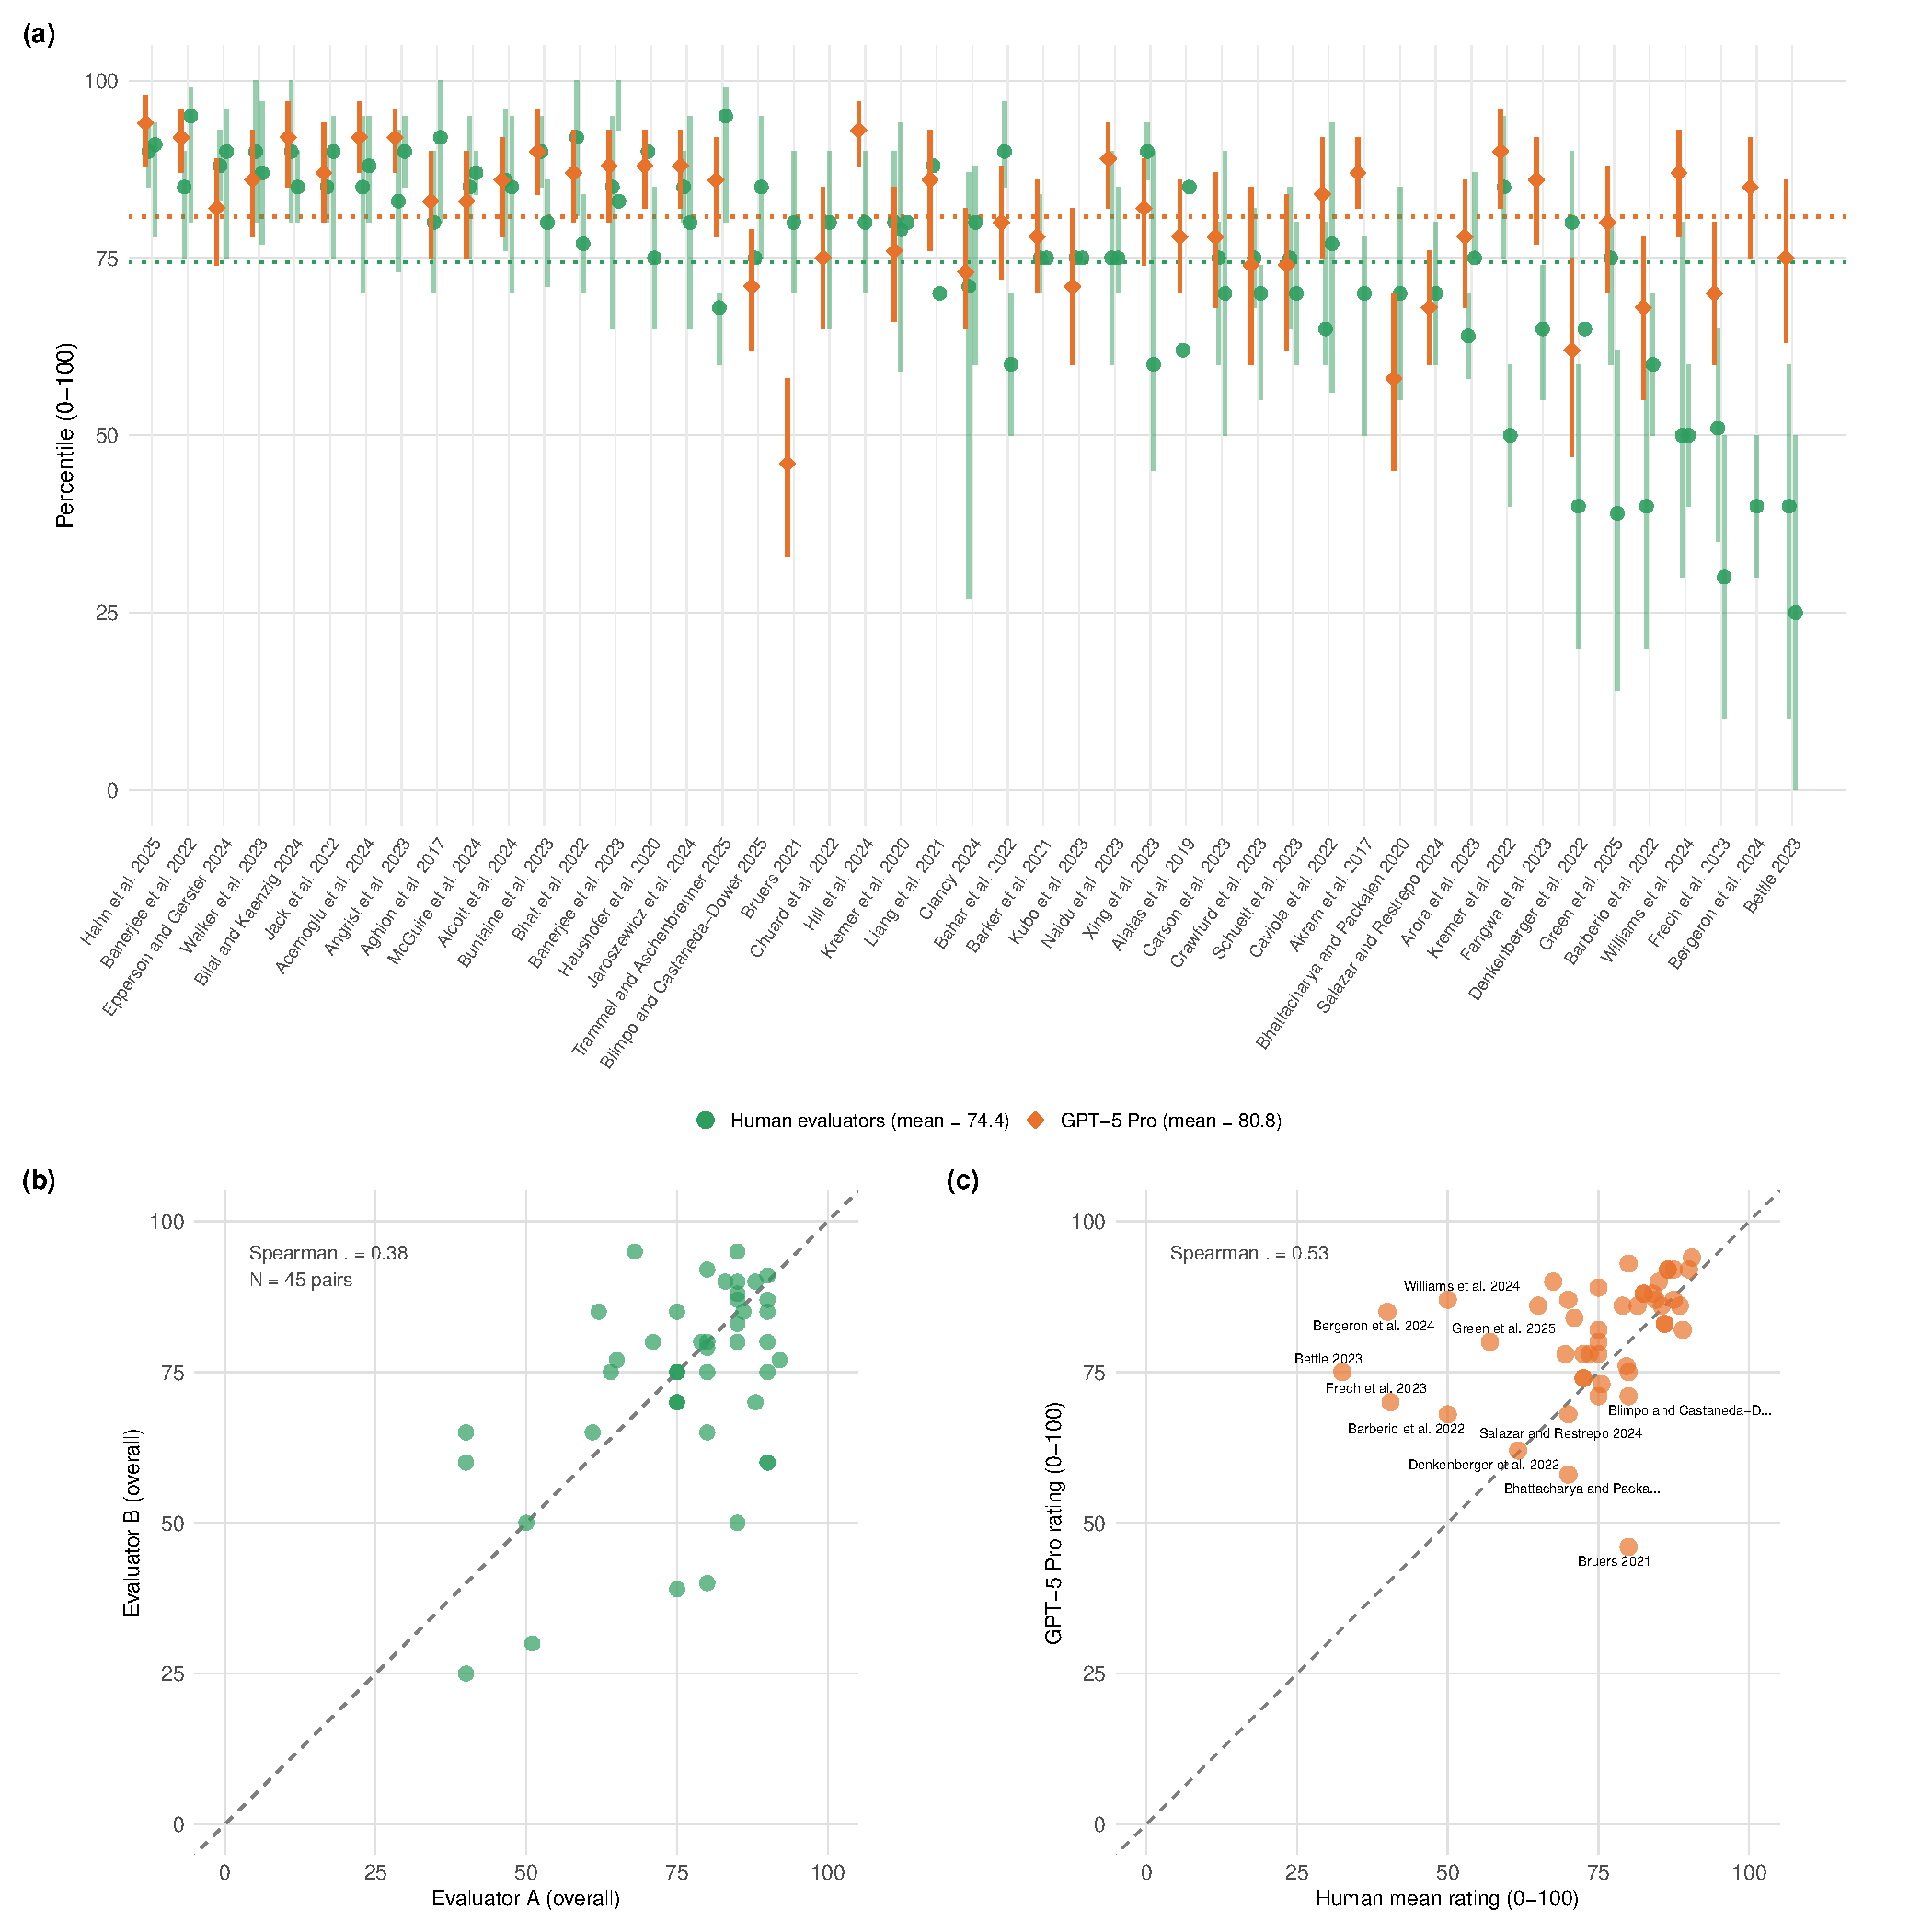
\includegraphics[keepaspectratio]{results_files/figure-pdf/fig-overview-combined-1.pdf}}

\end{figure}%

Both models cluster around the identity line in the 40--80 range but
diverge more at the extremes. LLMs tend to compress ratings toward the
centre of the scale relative to humans, producing narrower spread---a
pattern consistent with alignment training that discourages extreme
outputs. Where humans rate a paper very highly or very harshly, the LLM
typically pulls toward the middle. Full agreement metrics including
Pearson \emph{r}, Spearman \emph{ρ}, mean bias, and RMSE for all six
models appear in the \href{results_ratings.qmd}{agreement table in
Appendix A}.

\textbf{Rank comparison.} Figure~\ref{fig-rankslope-main} places human
rankings in the centre column with GPT-5 Pro on the left and Claude Opus
4.6 on the right, restricted to the 33 papers with Claude Opus 4.6
evaluations. Each paper appears as a pair of S-curves connecting its
human rank to its rank under each LLM. Horizontal curves indicate
agreement; curves that climb toward the top indicate the LLM ranked the
paper higher (better) than humans did. Colour encodes the rank shift:
green when humans rank it higher, orange (left, GPT-5 Pro) or purple
(right, Opus) when the LLM does. The triptych layout makes it easy to
spot papers where both LLMs agree with each other but disagree with
humans (both curves slope the same way), versus papers where the two
LLMs diverge.

\begin{figure}

\caption{\label{fig-rankslope-main}Triptych slopegraph of overall
ratings for the \texttt{r\ n\_papers\_slope}-paper matched sample
(papers evaluated by all three sources). Each column shows rank order (1
= highest rated) within that source; papers are connected by S-shaped
curves. Green = human panel ranks higher; orange (left) = GPT-5 Pro
ranks higher; purple (right) = Claude Opus ranks higher. Colour
intensity encodes magnitude of rank shift. Right-side labels show human
rank (H) and rank delta for each model (ΔG, ΔC; positive = LLM ranks
higher).}

\pandocbounded{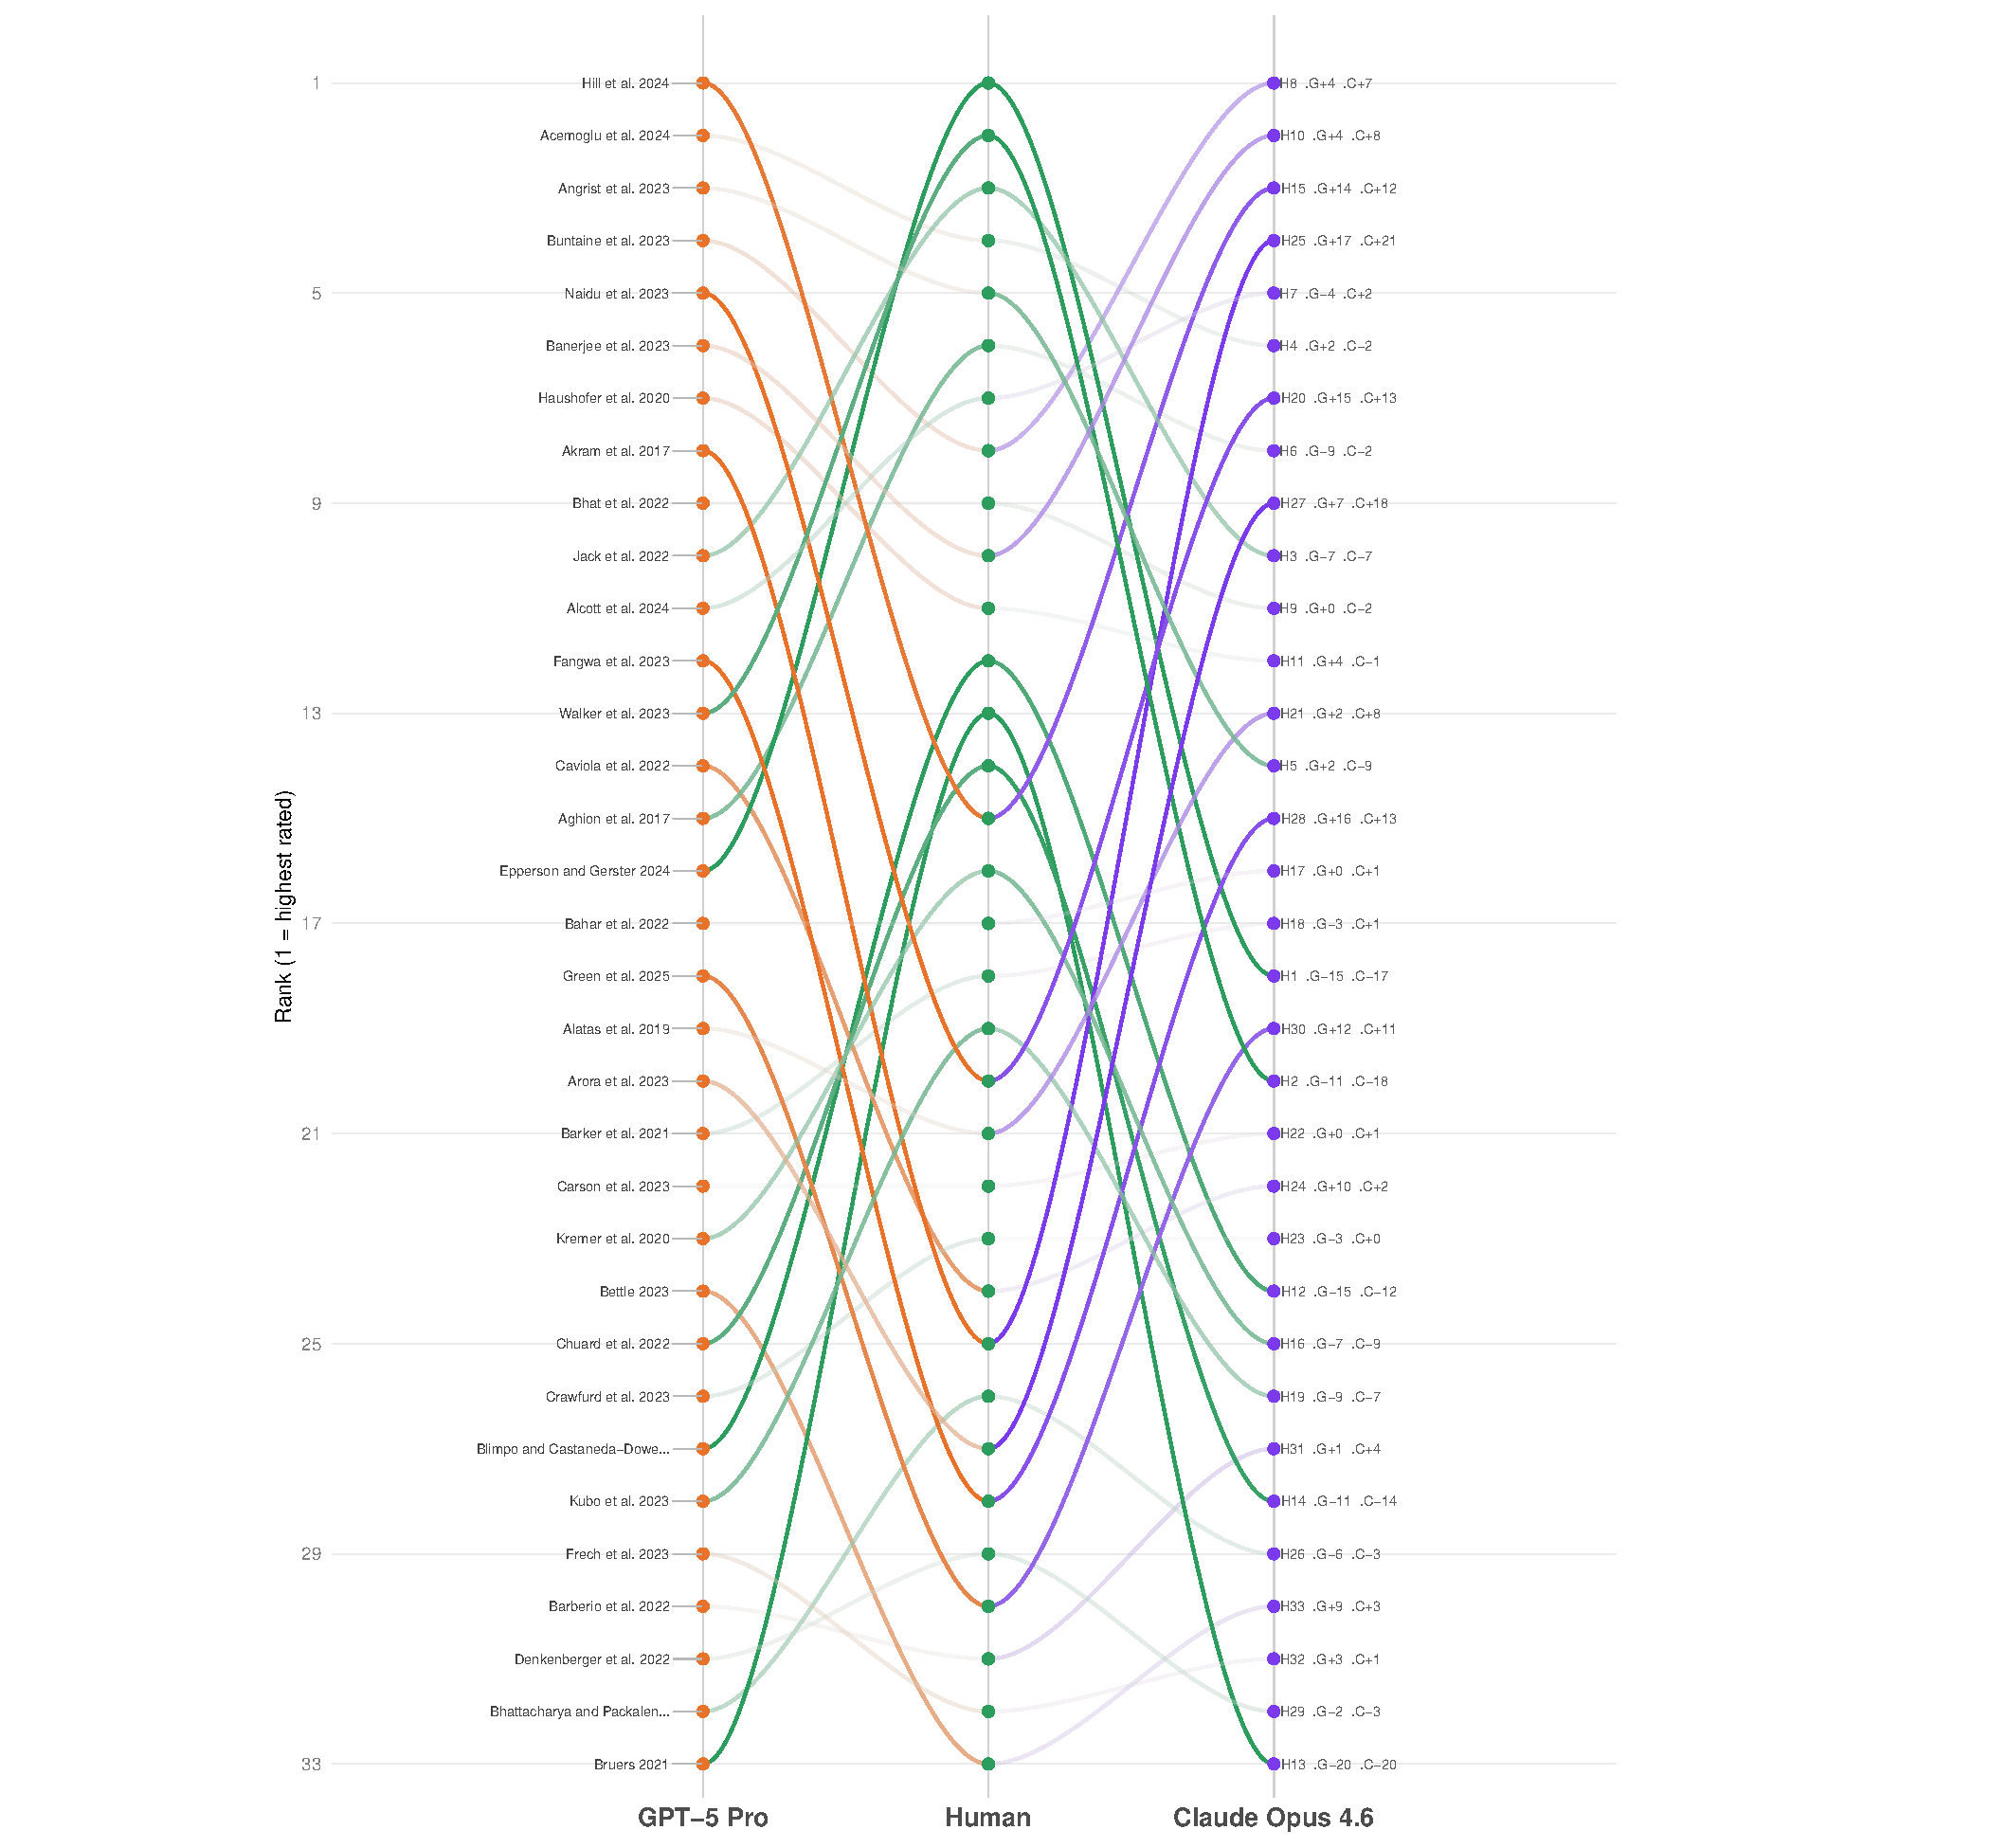
\includegraphics[keepaspectratio]{results_files/figure-pdf/fig-rankslope-main-1.pdf}}

\end{figure}%

Papers where both curves slope the same direction indicate systematic
human--LLM disagreement; papers where left and right curves diverge
indicate model-specific differences---GPT and Claude ``see'' the paper
differently, not just differently from humans. Horizontal curves
indicate agreement with the human ordering. The criteria-level
Krippendorff's alpha analysis in the \href{results_ratings.qmd}{human
baseline table in Appendix A} quantifies where human--LLM agreement
approaches the ceiling set by human inter-rater variability.

\textbf{Rating differences by paper and criterion.} While the scatter
plots and slopegraph summarise agreement on a single dimension,
Figure~\ref{fig-gap-heatmap-main} unpacks Human − LLM differences across
all seven criteria simultaneously. Each column is a paper, each row a
criterion, and tile colour encodes the signed difference (human mean
minus LLM midpoint). Green tiles indicate the human panel rated the
paper higher; orange (GPT-5 Pro) or purple (Claude Opus) tiles indicate
the LLM was more generous. Papers are sorted by GPT-5 Pro's overall
difference so that both panels share the same column order, making
model-specific patterns immediately visible.

\begin{figure}

\caption{\label{fig-gap-heatmap-main}Human minus LLM rating difference
for every paper (columns) and criterion (rows), comparing GPT-5 Pro
(left panel) and Claude Opus 4.6 (right panel). Green tiles indicate the
human mean was higher; orange (GPT-5 Pro) or purple (Claude Opus) tiles
indicate the LLM rated the paper higher. Colour is clamped to ±30
percentile points. Papers are sorted by GPT-5 Pro overall difference so
the two panels are directly comparable.}

\pandocbounded{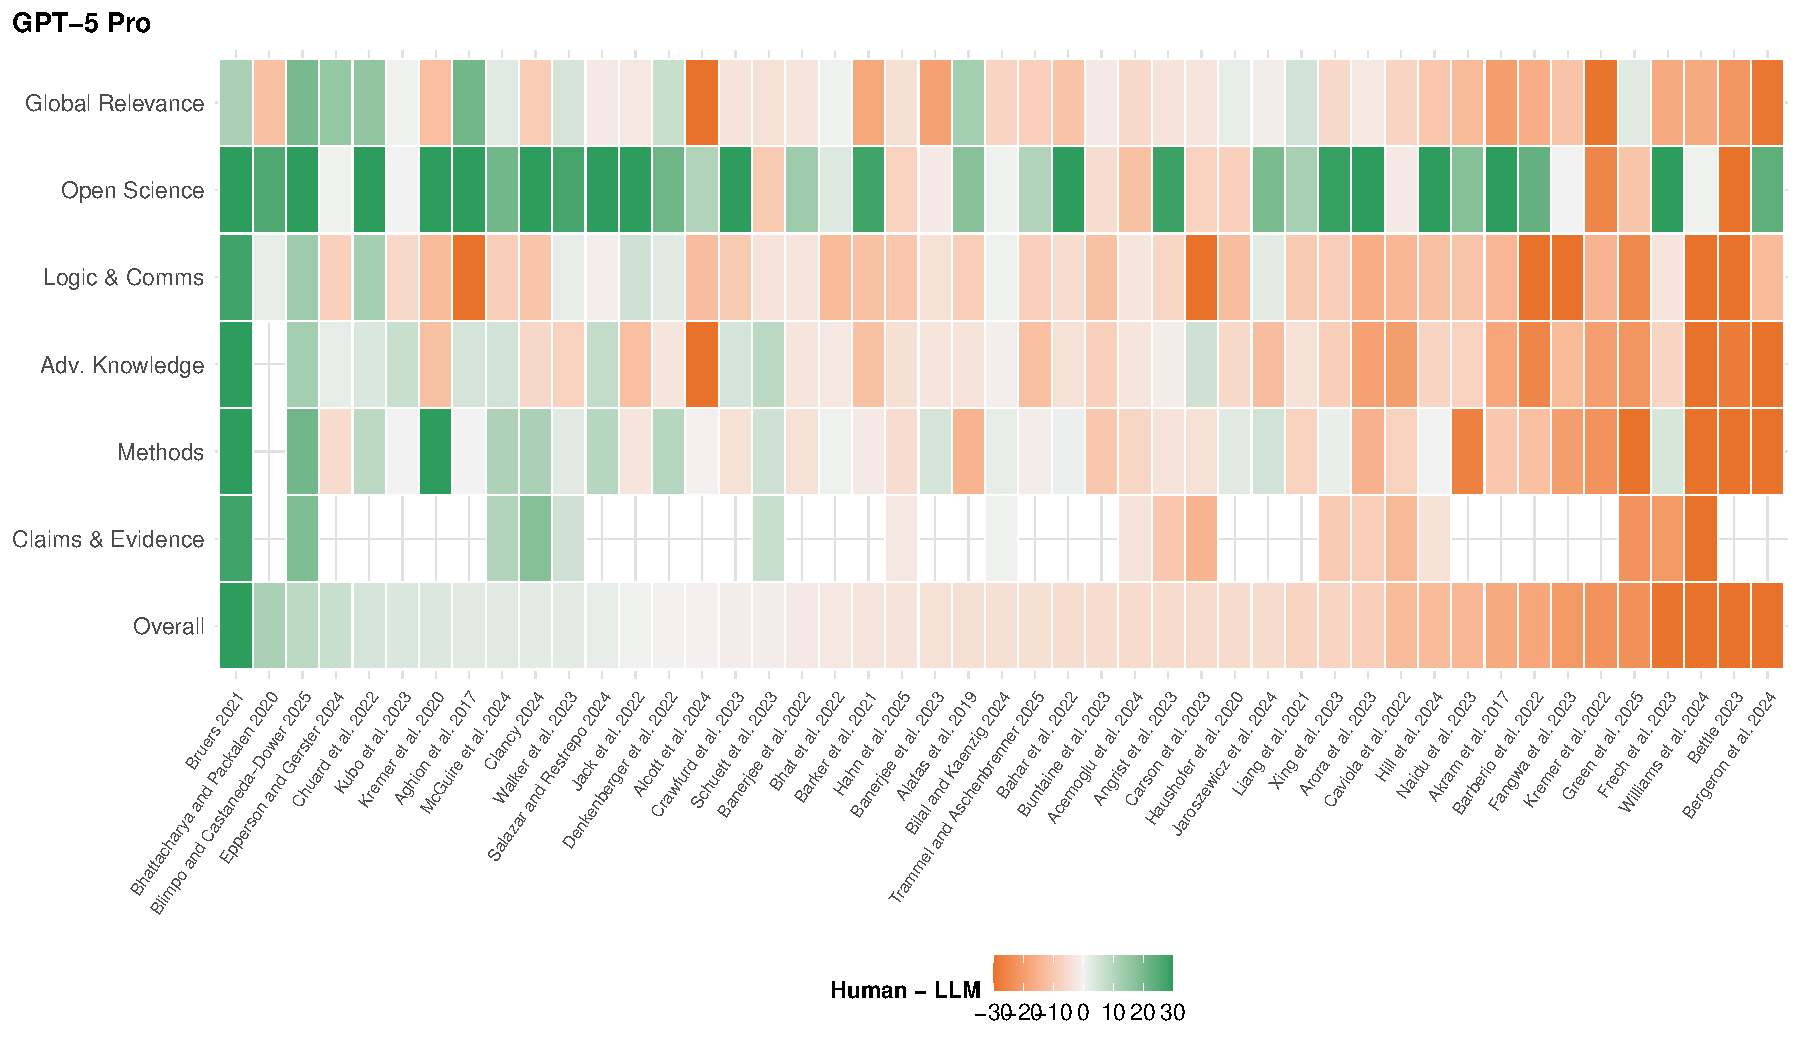
\includegraphics[keepaspectratio]{results_files/figure-pdf/fig-gap-heatmap-main-1.pdf}}

\end{figure}%

Rows with uniformly green or orange tiles indicate papers where humans
and the LLM disagree systematically across all criteria, not just on one
dimension. Columns with consistent colour suggest criteria-level
biases---for instance, if ``Open Science'' is green across nearly all
papers, humans may systematically reward data-sharing practices more
than the LLM does. Comparing the two panels reveals whether disagreement
patterns are model-specific or shared across frontier LLMs; tiles that
change colour between panels highlight papers where the models diverge
from each other, not just from humans.

\textbf{Qualitative critique comparison.} Beyond numeric ratings, we
compare the substantive critiques each model raises against the
consensus issues identified by human experts. The figure below plots
coverage---the fraction of human-identified concerns that the LLM also
raised in some form---against precision---the fraction of LLM-raised
issues that correspond to a substantive human concern. These metrics are
assessed by GPT-5.2 Pro acting as an independent judge (see
\href{methods.qmd}{Methods} for the judging protocol).

Coverage and precision vary substantially across papers. Some papers
achieve high scores on both dimensions, indicating strong alignment
between human and LLM critiques, while others reveal the LLM missing key
human concerns or raising issues absent from the expert consensus.
Because these metrics are themselves LLM-assessed, they should be
interpreted with the caveat that an LLM judge may systematically over-
or under-credit matches relative to a human annotator; manual validation
through our annotation tool is underway and preliminary results are
consistent with the automated scores.

Detailed paper-by-paper comparisons---including matched issue pairs with
severity labels, structural difference tables, and per-evaluator
breakdowns---appear in \href{results_critiques.qmd}{Appendix B:
Critiques \& Key Issues}. Extended quantitative analysis, including
per-criterion correlations, bootstrap confidence intervals, mutual
information, tier prediction accuracy, cost-quality trade-offs across
all six models, and top disagreement cases, is reported in
\href{results_ratings.qmd}{Appendix A: Results Ratings}. The full LLM
reasoning traces and assessment summaries are available in
\href{appendix_llm_traces.qmd}{Appendix C: LLM Traces}.

\textbf{Model comparison summary.} Table~\ref{tbl-model-agreement-main}
compares all six models on overall-rating agreement metrics against the
human mean, restricted to the 33-paper matched sample so every model is
evaluated on identical papers. Models are sorted by Pearson \emph{r}.

\begin{longtable}[]{@{}lrrrrrr@{}}

\caption{\label{tbl-model-agreement-main}Agreement between each LLM and
human mean overall rating (matched sample, N = \texttt{r\ n\_opus}
papers). Pearson \emph{r} and Spearman \emph{ρ} measure correlation;
bias = LLM − Human (positive = LLM more generous); RMSE and MAE measure
error magnitude. Models sorted by Pearson \emph{r}.}

\tabularnewline

\toprule\noalign{}
Model & N & Pearson r & Spearman ρ & Mean bias & RMSE & MAE \\
\midrule\noalign{}
\endhead
\bottomrule\noalign{}
\endlastfoot
Claude Opus 4.6 & 33 & 0.567 & 0.477 & -7.6 & 17.2 & 12.4 \\
Gemini 2.0 Flash & 33 & 0.467 & 0.447 & -5.3 & 13.2 & 10.8 \\
GPT-5.2 Pro & 5 & 0.433 & 0.410 & -6.6 & 19.9 & 15.4 \\
GPT-5 Pro & 33 & 0.396 & 0.553 & +5.1 & 14.1 & 10.0 \\
GPT-4o-mini & 33 & 0.356 & 0.309 & -0.1 & 15.9 & 10.7 \\
Claude Sonnet 4 & 8 & -0.232 & -0.058 & -1.6 & 9.1 & 6.8 \\

\end{longtable}

Table~\ref{tbl-criteria-agreement-main} breaks the same agreement
metrics down by evaluation criterion, averaged across all models in the
matched sample, to reveal which dimensions of research quality show
stronger vs weaker human--LLM alignment.

\begin{longtable}[]{@{}lrrrr@{}}

\caption{\label{tbl-criteria-agreement-main}Human--LLM agreement by
criterion, averaged across all models (matched sample, N =
\texttt{r\ n\_opus} papers). Higher Pearson \emph{r} indicates better
alignment; positive bias indicates LLMs are more generous on that
criterion.}

\tabularnewline

\toprule\noalign{}
Criterion & Pearson r & Spearman ρ & Mean bias & RMSE \\
\midrule\noalign{}
\endhead
\bottomrule\noalign{}
\endlastfoot
Overall & 0.415 & 0.406 & -2.1 & 15.1 \\
Claims \& Evidence & 0.362 & 0.279 & -4.5 & 16.9 \\
Methods & 0.304 & 0.323 & -1.2 & 18.4 \\
Adv. Knowledge & 0.230 & 0.218 & +1.1 & 16.8 \\
Logic \& Comms & 0.082 & 0.041 & +3.9 & 16.9 \\
Open Science & 0.037 & 0.008 & -11.7 & 27.0 \\
Global Relevance & 0.181 & 0.257 & -0.3 & 17.6 \\

\end{longtable}

All appendices, interactive figures, and full code are available at the
companion website: \url{https://llm-uj-research-eval.netlify.app}.
Source code and data are hosted at
\url{https://github.com/valentinklotzbuecher/llm-uj-research-eval}.

\bookmarksetup{startatroot}

\section{Discussion}\label{discussion}

Frontier LLMs achieve moderate-to-strong agreement with human expert
evaluators, approaching the ceiling set by inter-rater variability among
humans themselves. Correlations with human mean ratings are highest for
reasoning-capable models (GPT-5 Pro, Claude Opus 4.6), though even
lightweight models (GPT-4o-mini, Gemini 2.0 Flash) perform respectably
at a fraction of the cost. Central compression---the tendency for LLMs
to pull extreme ratings toward the middle of the scale---is the most
consistent pattern across all models, likely reflecting alignment
training that discourages confident extreme outputs. Qualitative
coverage varies widely across papers: on some, the LLM captures nearly
all consensus human concerns; on others, it misses key critiques or
raises issues absent from the expert consensus.

\textbf{Limitations.} Several caveats temper these conclusions. Our
sample comprises roughly 50 social-science papers specifically selected
by The Unjournal for evaluation, not a random draw from the research
literature; performance may differ in other fields or on less polished
manuscripts. Human evaluations are themselves a noisy reference signal
rather than ground truth, with substantial inter-rater variation that
caps achievable agreement. We cannot fully rule out knowledge
contamination: while we block extrinsic priors in the system prompt, the
models' training data may include fragments of these papers or related
discussions. Alignment training likely contributes to score inflation
and narrower credible intervals than humans provide. All LLM evaluations
are single-run; aggregating across multiple runs or temperature settings
could change the picture. Finally, the qualitative coverage and
precision metrics are themselves LLM-assessed (GPT-5.2 Pro as judge),
introducing a further layer of model dependence.

\textbf{Implications.} The cost structure is striking: lightweight
models deliver evaluations at under a cent per paper, while
reasoning-capable models cost several dollars---still orders of
magnitude cheaper than human expert review. This suggests a practical
tier structure in which cheap models could serve as rapid screening
tools and expensive reasoners could provide deeper assessment where
warranted. However, the qualitative gaps we observe---missed critiques,
generic issues, and central compression of ratings---argue against full
automation of peer review. AI evaluation appears most promising as a
supplement: providing fast structured feedback, flagging potential
concerns for human reviewers, and enabling systematic comparison across
large paper sets that would be infeasible with human effort alone.

\textbf{Governance and attack surface.} As AI review tools move from
research prototypes to deployed products, the attack surface expands.
Prompt-injection techniques---embedding hidden instructions in a
manuscript's metadata, footnotes, or even white-on-white text---could
steer model outputs toward inflated ratings or suppressed critiques.
Because our pipeline (and similar commercial services) routes
unpublished manuscripts through third-party APIs, confidentiality cannot
be guaranteed without end-to-end encryption or on-premise deployment.
Over-reliance on AI scores introduces a further governance risk: if
editorial decisions weight model ratings, authors may optimise papers
for the model rather than for scientific rigour, creating a Goodhart
dynamic. Finally, current evaluations reflect a single model checkpoint;
model updates, alignment changes, or fine-tuning can shift ratings in
ways that are invisible to users. We recommend that any operational
deployment include adversarial red-teaming of prompts, formal
confidentiality agreements with API providers, transparent disclosure of
AI involvement in review, and periodic re-calibration against fresh
human evaluations.

\textbf{Future work.} Several extensions follow naturally from this
analysis. Content-swap bias tests following Pataranutaporn et al.
(\citeproc{ref-Pataranutaporn2025}{2025}) would reveal whether LLMs show
systematic biases based on author names or institutional affiliations. A
journal-outcome prediction horse-race would compare human and LLM tier
predictions against actual publication venues. Systematic prompt and
model comparisons, including agent-based approaches, could identify
configurations that reduce central compression or improve qualitative
coverage. Human enumerator validation---employing trained raters to
independently assess whether LLMs identify the same consensus
critiques---would ground the currently LLM-assessed coverage metrics.
Out-of-time validation using papers entering The Unjournal's pipeline
would eliminate contamination concerns entirely. Finally, hybrid
human-AI evaluation trials would test whether collaboration improves
evaluation quality beyond either alone.

\bookmarksetup{startatroot}

\section{Methods}\label{methods}

\small

This chapter describes the data sources, evaluation pipeline, prompt
design, and statistical methods used throughout. All Python code
underlying the pipeline is preserved in the collapsible blocks below and
can be executed to reproduce the evaluation runs.

\textbf{Sample and human reference data.} We draw on published
evaluations from
\href{https://unjournal.github.io/unjournaldata/index.html}{The
Unjournal}, an open-access platform that commissions expert reviews of
policy-relevant research without requiring journal submission. Each
paper is typically assessed by two independent evaluators (occasionally
one or three), who provide a written critique resembling a referee
report together with quantitative ratings on seven criteria scored as
percentiles (0--100) relative to ``all serious research in the same area
encountered in the last three years.''\footnote{The seven criteria are:
  \emph{overall assessment}, \emph{claims and evidence}, \emph{methods},
  \emph{advancing knowledge and practice}, \emph{logic and
  communication}, \emph{open and collaborative science}, and
  \emph{relevance to global priorities}. Full definitions are given in
  The Unjournal's
  \href{https://globalimpact.gitbook.io/the-unjournal-project-and-communication-space/policies-projects-evaluation-workflow/evaluation/guidelines-for-evaluators}{guidelines
  for evaluators}.} Evaluators additionally predict the journal tier in
which the work ``should'' and ``will'' publish, using a 0--5 continuous
scale anchored to familiar venue categories (0 = unpublishable, 5 =
top-5 journal). For each metric, evaluators report a midpoint (median of
their belief distribution) and a 90\% credible interval that expresses
their epistemic uncertainty.

The sample comprises working papers spanning 2017--2025 in development
economics, health policy, environmental economics, and related fields
that The Unjournal identified as high-impact. All papers have completed
The Unjournal's full evaluation process, meaning the authors received
evaluations that have been publicly posted. For our analysis we
extracted the individual evaluator scores, aggregated them by taking the
arithmetic mean per paper per criterion, and retained the range of
individual scores to characterise inter-rater spread.

\textbf{LLM evaluation pipeline.} We evaluate six frontier models
spanning three providers: GPT-5 Pro and GPT-5.2 Pro (OpenAI,
reasoning-capable), GPT-4o-mini (OpenAI, lightweight), Claude Sonnet 4
and Claude Opus 4.6 (Anthropic), and Gemini 2.0 Flash (Google). Each
model receives the identical PDF file, system prompt, and output schema.
We pass the PDF directly to the model's native multimodal input rather
than extracting text, preserving tables, figures, equations, and layout
cues that ad-hoc scraping could mangle. A single API call per paper
avoids hand-offs and summary loss from multi-stage pipelines.

The output is constrained by a strict JSON Schema enforcing the same
nine fields that human evaluators complete: seven percentile metrics
(each with \texttt{midpoint}, \texttt{lower\_bound},
\texttt{upper\_bound}) and two journal-tier predictions (each with
\texttt{score}, \texttt{ci\_lower}, \texttt{ci\_upper}). Additionally,
the model produces an \texttt{assessment\_summary} of approximately
1,000 words that must precede scoring---a ``think first, score second''
protocol designed to ground numeric ratings in specific textual
evidence. The extended schema used for our GPT-5.2 Pro focal run adds a
\texttt{key\_issues} array of concise, ranked issue statements for
downstream critique comparison.

\textbf{Agreement and reliability statistics.} We quantify human--LLM
agreement using several complementary measures. \emph{Pearson's r}
captures linear association between paired ratings and is sensitive to
proportional biases but not to constant offsets. \emph{Spearman's ρ}
measures rank-order agreement and is robust to outliers and non-linear
monotone relationships. \emph{Mean bias} (LLM minus human) indicates the
direction and magnitude of any systematic offset. \emph{Root mean
squared error} (RMSE) and \emph{mean absolute error} (MAE) measure
typical prediction error in the original scale units; RMSE penalises
large deviations more heavily. To contextualise human--LLM agreement we
report \emph{Krippendorff's alpha} (\(\alpha\)), a chance-corrected
reliability coefficient that generalises across varying numbers of
raters, accommodates missing data, and applies to any measurement level
(nominal, ordinal, interval, or ratio). An \(\alpha\) of 1 indicates
perfect agreement, 0 indicates agreement no better than chance, and
values below 0 indicate systematic disagreement. We compute
\(\alpha_{\text{HH}}\) (among human evaluators only) as a ceiling: if
human evaluators agree with each other at only \(\alpha = 0.5\) on a
given criterion, expecting an LLM to exceed that level would be
unrealistic. We then report \(\alpha_{\text{HL}}\) (between the human
mean and each LLM) to assess how close machine ratings come to this
ceiling. For the qualitative key-issue comparison, \emph{coverage}
denotes the fraction of human-identified issues that received a match
score \(\geq 30\%\) from the LLM judge, and \emph{precision} denotes the
fraction of LLM-generated issues that matched at least one human issue.

\textbf{JSON Schema.} The output schema enforces that every paper is
scored on identical fields with identical types and bounds. Credible
intervals are required (paralleling the human protocol) so that the
model can express genuine uncertainty rather than suggest false
precision.

\textbf{System prompt design.} The system prompt is assembled from
modular components and concatenated before each API call. It opens with
a role definition instructing the model to act as an expert research
evaluator, followed by a debiasing block that explicitly prohibits use
of author identity, institutional prestige, publication venue, or any
extrinsic information---the model must base all judgments on the PDF
content alone. A diagnostic-summary instruction requires the model to
produce a roughly 1,000-word assessment identifying methodological,
evidential, and interpretive issues \emph{before} any scoring,
implementing a ``think first, score second'' protocol intended to anchor
numeric ratings in specific textual evidence.

Percentile ratings are anchored to the reference group ``all serious
research in the same area encountered in the last three years,''
following The Unjournal's
\href{https://globalimpact.gitbook.io/the-unjournal-project-and-communication-space/policies-projects-evaluation-workflow/evaluation/guidelines-for-evaluators}{guidelines
for evaluators}. The prompt defines each of the seven criteria with
emphasis on global priorities and practical relevance over pure academic
novelty, mirroring the weight structure that human Unjournal evaluators
are asked to apply.

Subsequent prompt components instruct the model on constructing 90\%
credible intervals---the smallest interval the evaluator believes is
90\% likely to contain the true value---encouraging calibrated
uncertainty rather than artificially narrow bounds. The prompt requests
journal-tier predictions on a 0--5 continuous scale anchored to familiar
venue categories (0 = unpublishable through 5 = top-5 journal),
providing an externally verifiable reference point for papers that
eventually publish. A validation block then requires the model to verify
internal consistency: numeric scores must align with the written
assessment, credible intervals must be non-degenerate, and high or low
ratings must be explicitly justified in the assessment summary.

The components above are concatenated into a single system prompt string
before each API call:

\textbf{Submission and collection.} The \texttt{evaluate\_paper}
function uploads a PDF to the API and submits a background job for
evaluation. File IDs are cached by path, size, and modification time so
that re-running on the same PDF reuses the previously uploaded file.

Each model receives the full PDF in a single reasoning call, avoiding
hand-offs and summary loss from multi-stage ingestion. We submit one
background job per paper to the OpenAI Responses API with ``high''
reasoning effort and server-side JSON-Schema enforcement, recording the
response ID, model, file ID, status, and timestamps in a jobs index. No
external sources or cross-paper material are retrieved; the evaluation
is anchored entirely in the manuscript itself.

A polling loop then checks each job's status and, for completed jobs,
retrieves the raw JSON response object and writes it to disk alongside
reasoning-trace metadata (token counts, reasoning summary).

\textbf{Multi-model evaluation.} To assess whether systematic biases or
calibration differences emerge across architectures, we collect
evaluations from six models spanning three providers. For OpenAI models
that lack background-job or extended-reasoning support (e.g.,
GPT-4o-mini), we use a synchronous call variant:

\textbf{Anthropic.} Anthropic's API accepts PDFs as base64-encoded
document content rather than uploaded file IDs, and all calls are
synchronous. We use Claude's native PDF support to preserve the same
multimodal evaluation approach:

\textbf{Google.} Google's Gemini API accepts PDFs via a file-upload
endpoint with MIME-type tagging:

A unified runner dispatches evaluations across all configured providers
and writes per-model output directories:

\textbf{Focal run with key-issue extraction.} For a subset of 14 papers
with rich human critiques, we ran an extended evaluation using GPT-5.2
Pro. The schema for this focal run adds a \texttt{key\_issues} array---a
ranked list of concise issue statements identifying the most important
methodological, interpretive, or evidential concerns---alongside the
standard metrics. This structured output enables direct comparison
between machine-generated and human-identified issues.

\textbf{Key-issue comparison with human critiques.} To validate how well
the LLM identifies substantive concerns, we compare its
\texttt{key\_issues} output against human expert critiques drawn from
The Unjournal's Coda database. These human critiques---produced by paid
domain experts and synthesized by evaluation managers---provide a
high-quality but noisy reference standard for issue identification;
accordingly, we treat them as a comparative signal rather than ground
truth.

The comparison proceeds in two stages. First, we parse and align the
data sources: LLM key issues are extracted from the focal-run JSON
responses, while human critiques are drawn from a manually curated
markdown document pairing each paper's machine and expert assessments.
Second, we use an LLM judge (GPT-5.2 Pro with schema-enforced structured
output) to systematically assess the degree of alignment between each
human-identified issue and the set of machine-generated issues,
producing issue-by-issue match scores, coverage estimates (fraction of
human issues captured), and precision estimates (fraction of LLM issues
that are genuinely substantive).

The comparison pipeline takes a manually curated markdown file pairing
each paper's LLM issues with human critiques and produces two structured
outputs: a parsed JSON dataset (\texttt{key\_issues\_comparison.json})
and an LLM-assessed alignment report
(\texttt{key\_issues\_comparison\_results.json}) containing per-paper
coverage, precision, matched-pair explanations, and an overall quality
rating. Together, these outputs feed the qualitative analysis presented
in \href{results_critiques.qmd}{Appendix B: Critiques \& Key Issues}.

\normalsize

\bookmarksetup{startatroot}

\section*{References}\label{references}
\addcontentsline{toc}{section}{References}

\markboth{References}{References}

\phantomsection\label{refs}
\begin{CSLReferences}{1}{0}
\bibitem[\citeproctext]{ref-aczel2021billion}
Aczel, Balazs, Barnabas Szaszi, and Alex O Holcombe, {``A billion-dollar
donation: Estimating the cost of researchers' time spent on peer
review,''} \emph{Research integrity and peer review}, 6 (2021), 1--8
(Springer).

\bibitem[\citeproctext]{ref-AsherMalzahnPersanoPaschalMyersHall2026P_Hack}
Asher, Samuel G. Z., Janet Malzahn, Jessica M. Persano, Elliot J.
Paschal, Andrew C. W. Myers, and Andrew B. Hall, {``Do claude code and
codex p-hack? {Sycophancy} and statistical analysis in large language
models,''} 2026.

\bibitem[\citeproctext]{ref-AsirvathamMokskiShleifer2026GPTMeasurement}
Asirvatham, Hemanth, Elliott Mokski, and Andrei Shleifer,
{``\href{https://www.nber.org/papers/w34834}{{GPT} as a measurement
tool},''} \{NBER\} Working Paper, 2026 (National Bureau of Economic
Research).

\bibitem[\citeproctext]{ref-choi2026invisible}
Choi, Byungjin, Tae Joon Jun, Joung Won Sung, Il Woo Park, Jeong-Moo
Lee, Soo Ick Cho, Hyung Jun Park, Ro Woon Lee, and Jungyo Suh,
{``\href{https://doi.org/10.1001/jamanetworkopen.2025.52099}{Invisible
text injection and peer review by AI models},''} \emph{JAMA Network
Open}, 9 (2026), e2552099.

\bibitem[\citeproctext]{ref-elsevierAIPolicy2025}
Elsevier,
{``\href{https://www.elsevier.com/about/policies-and-standards/generative-ai-policies-for-journals}{Generative
AI policies for journals}''} (Feb. 19, 2026).

\bibitem[\citeproctext]{ref-isitcredible}
IsItCredible.com, {``\href{https://www.isitcredible.com/}{Is it
credible?}''} (Feb. 19, 2026).

\bibitem[\citeproctext]{ref-lee2025promptinj}
Lee, Ro Woon, Tae Joon Jun, Jeong-Moo Lee, Soo Ick Cho, Hyung Jun Park,
and Jungyo Suh,
{``\href{https://doi.org/10.1001/jamanetworkopen.2025.49963}{Vulnerability
of large language models to prompt injection when providing medical
advice},''} \emph{JAMA Network Open}, 8 (2025), e2549963.

\bibitem[\citeproctext]{ref-leung2026policies}
Leung, Tiffany I.,
{``\href{https://doi.org/10.1001/jamanetworkopen.2025.52042}{LLMs in
peer review---how publishing policies must advance},''} \emph{JAMA
Network Open}, 9 (2026), e2552042.

\bibitem[\citeproctext]{ref-Pataranutaporn2025}
Pataranutaporn, Pat, Nattavudh Powdthavee, Chayapatr Achiwaranguprok,
and Pattie Maes, {``\href{https://doi.org/10.48550/arXiv.2502.00070}{Can
AI solve the peer review crisis? A large scale cross model experiment of
LLMs' performance and biases in evaluating over 1000 economics
papers},''} 2025.

\bibitem[\citeproctext]{ref-rajakumar2026peerreview}
Rajakumar, Hamrish Kumar, Kailash Abhishek Sankaran, Manasi Pillai
Ashok, and Srinivas Rachoori,
{``\href{https://doi.org/10.1093/postmj/qgag005}{Peer review in the age
of artificial intelligence: A comparative study of human and
AI-generated review reports},''} \emph{Postgraduate Medical Journal},
(2026), qgag005.

\bibitem[\citeproctext]{ref-refineFAQ}
Refine, {``\href{https://www.refine.ink/faq}{FAQ - refine}''} (Feb. 19,
2026).

\bibitem[\citeproctext]{ref-spitzer2026submission}
Spitzer, Markus Wolfgang Hermann,
{``\href{https://doi.org/10.1016/j.tine.2026.100276}{The emerging
submission crisis in behavioral science},''} \emph{Trends in
Neuroscience and Education}, 42 (2026), 100276.

\bibitem[\citeproctext]{ref-thomas2026jagged}
Thomas, Llewellyn D. W., Angelo Kenneth G. Romasanta, and Laia Pujol
Priego, {``\href{https://doi.org/10.1016/j.jbusres.2025.115804}{Jagged
competencies: Measuring the reliability of generative AI in academic
research},''} \emph{Journal of Business Research}, 203 (2026), 115804.

\bibitem[\citeproctext]{ref-wang2025psychometric}
Wang, Yuehan, Jinyan Huang, Lun Du, Yuxin Guo, Ying Liu, and Rong Wang,
{``\href{https://doi.org/10.1016/j.caeai.2025.100481}{Evaluating large
language models as raters in large-scale writing assessments: A
psychometric framework for reliability and validity},''} \emph{Computers
and Education: Artificial Intelligence}, 9 (2025), 100481.

\bibitem[\citeproctext]{ref-xu2026scaling}
Xu, Yiqing, and Leo Y. Yang,
{``\href{https://yiqingxu.org/papers/2026_ai/AI_reproducibility.pdf}{Scaling
reproducibility: An AI-assisted workflow for large-scale reanalysis},''}
2026.

\bibitem[\citeproctext]{ref-Zhang2025}
Zhang, Tianmai M, and Neil F Abernethy,
{``\href{https://arxiv.org/abs/2505.23824v2}{Reviewing scientific papers
for critical problems with reasoning LLMs: Baseline approaches and
automatic evaluation},''} \emph{arXiv preprint arXiv:2505.23824},
(2025).

\end{CSLReferences}

\cleardoublepage
\phantomsection
\addcontentsline{toc}{part}{Appendices}
\appendix

\section{Results: Ratings}\label{results-ratings}

Extended ratings analysis (per-criterion correlations, agreement
metrics, human baseline, cost--quality trade-offs) is available in the
online supplement at
\url{https://llm-uj-research-eval.netlify.app/results_ratings.html}.

\section{Results: Critiques \& Key
Issues}\label{results-critiques-key-issues}

Detailed paper-by-paper critique comparisons (matched issue pairs,
severity labels, structural differences) are available in the online
supplement at
\url{https://llm-uj-research-eval.netlify.app/results_critiques.html}.

\section{Supplementary Material}\label{supplementary-material}

Full LLM reasoning traces, assessment summaries, related work, and
extended analyses are available in the online supplement at
\url{https://llm-uj-research-eval.netlify.app/appendix_llm_traces.html}.




\end{document}
